% !TeX root = main.tex

\hypertarget{derivatives-as-rates-of-change}{%
\section{Derivatives as Rates of
Change}\label{derivatives-as-rates-of-change}}

If \(f(x)\) is a function defined on a small interval \([a, a+h]\), then
the amount of change of \(f(x)\) over the interval \(f(a+h)-f(a)\) is
approximately \(f'(a)h\) if \(f\) is differentiable at \(a\). This is
because
\[\lim\limits_{h\to 0}h\cdot\left(\dfrac{f(a+h)-f(a)}{h}-f'(a)\right)=0\]
which means \(f(a+h)-f(a)-f'(a)h\) can be arbitrarily small as long as
\(h\) is small enough.

\begin{fullwidth}
  \centering
  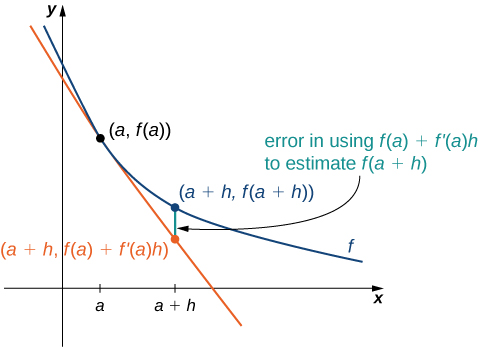
\includegraphics{img/DerivativeRateChange.png}
\end{fullwidth}

\hypertarget{motion-along-a-line}{%
\subsection{Motion Along a Line}\label{motion-along-a-line}}

\textbf{Definition:} Suppose an object is moving along a coordinate
line. Let \(s(t)\) be a function giving the position of the object at
time \(t\).

\begin{itemize}
\item
  The \textbf{displacement} of the object over the time interval from
  \(t\) to \(t+\Delta t\) is \(\Delta s=s(t+\Delta t)+s(t)\), where
  \(\Delta t\) is an increment of time.
\item
  The \textbf{average velocity} of the object over a time interval from
  \(t\) to \(t+\Delta t\) is \(v_{ave}=\dfrac{\Delta s}{\Delta t}\).
\item
  The \textbf{velocity (instantaneous velocity)} of the object at time
  \(t\) is given by
  \(v(t)=\lim\limits_{\Delta t\to 0}\dfrac{\Delta s}{\Delta t}=s'(t)\).
\item
  The \textbf{speed} of the object at time \(t\) is given by \(|v(t)|\).
\item
  The \textbf{acceleration} of the object at \(t\) is given by
  \(a(t)=v'(t)=s''(t)\).
\end{itemize}

\begin{example}

A ball is dropped from a height of 64 feet. Its height above ground (in
feet) \(t\) seconds later is given by \(s(t)=-16t^2+64\).

\begin{enumerate}
\item
  What is the velocity of the ball when it hits the ground?
\item
  When is the object at rest?
\end{enumerate}

\end{example}
% \vspace*{6\baselineskip}

\begin{example}

A particle moves along a coordinate axis. Its position at time \(t\) is given by
\(s(t)=t^3-9t^2+24t+4\).

\begin{enumerate}
\item
  Find \(v(t)\) and \(a(t)\) and use these values to answer the
  following questions.
\item
  On what time intervals is the particle moving from left to right?
\item
  On what time intervals is the particle moving from right to left?
\end{enumerate}

\end{example}
% \vspace*{6\baselineskip}

\hypertarget{population-change}{%
\subsection{Population Change}\label{population-change}}

\begin{definition}

If \(P(t)\) is the number of entities present in a population, then the
\textbf{population growth rate} of \(P(t)\) is defined to be \(P'(t)\).

\end{definition}

\begin{example}

The population of a city is tripling every 5 years. If its current
population is 10,000, what will be its approximate population 2 years
from now?

\end{example}
\vspace*{6\baselineskip}

\hypertarget{derivative-in-economics}{%
\subsection{Derivative in Economics}\label{derivative-in-economics}}

\begin{itemize}
\item
  If \(C(x)\) is the cost of producing \(x\) items, then the
  \textbf{marginal cost} \(MC(x)\) is \(MC(x)=C'(x)\).
\item
  If \(R(x)\) is the revenue obtained from selling \(x\) items, then the
  \textbf{marginal revenue} \(MR(x)\) is \(MR(x)=R'(x)\).
\item
  If \(P(x)=R(x)-C(x)\) is the profit obtained from selling \(x\) items,
  then the \textbf{marginal profit} \(MP(x)\) is defined to be
  \(MP(x)=P'(x)=MR(x)-MC(x)=R'(x)-C'(x)\).
\end{itemize}


\begin{example}

Suppose that the profit obtained from the sale of \(x\) fish-fry dinners is given by \(P(x)=-0.03x^2+8x-50\). Use the marginal profit function to estimate the profit from the sale of the 101st fish-fry dinner.

\end{example}
\vspace*{6\baselineskip}

\subsection{Practice}

\begin{exercise}
  A particle moves along a coordinate axis. Its position at time  t  is given by $s(t)=t^2-5t+1$ . Is the particle moving from right to left or from left to right at time  $t=3$?
\end{exercise}
\vspace*{6\baselineskip}

\begin{exercise}

  A particle moves along a coordinate axis. Its position at time \(t\) is given by
  \(s(t)=t^3-8t\).
  
  \begin{enumerate}
  \item
    Determine the direction the particle is traveling when $s(t)=0$.
  \item
    On what time intervals is the particle moving from right to left?
  \item
    Determine the direction the train is traveling when $a(t)=0$?
  \end{enumerate}
  
\end{exercise}


\begin{exercise}

The current population of a mosquito colony is known to be 3,000; that
is, \(P(0)=3,000\). If \(P'(0)=100\), estimate the size of the
population in 3 days, where \(t\) is measured in days.

\end{exercise}
\vspace*{6\baselineskip}

\begin{exercise}

The cost (in dollars) of producing \(x\) units of a certain commodity is
\(C(x) = 20 + 100\sqrt{x} + 0.01x^2\).

\begin{enumerate}
\item
  Find the marginal cost function.
\item
  Find \(C'(100)\) and explain it meaning.
\item
  What is the difference between \(C'(100)\) and the additional cost for
  producing the 1001st commodity?
\end{enumerate}

\end{exercise}

